%%&../../myformat
\documentclass[fleqn,leqno,10pt,letterpaper,final]{article}
%----README----
% This TeX file was automatically generated by GNU Emacs's Org Mode.
% For better documentation refer to the corresponding Org file, 
% which you can find in the sources specified bellow.
% Do keep in mind that this file undergoes little to none manual revision.
%----LICENSE---
% Copyright 2021 Jhonny Lanzuisi (jalb97@gmail.com)
% More source files at github.com/JLanzuisi
%
% This program is free software: you can redistribute it and/or modify
% it under the terms of the GNU General Public License as published by
% the Free Software Foundation, either version 3 of the License, or
% (at your option) any later version.
%
% This program is distributed in the hope that it will be useful,
% but WITHOUT ANY WARRANTY; without even the implied warranty of
% MERCHANTABILITY or FITNESS FOR A PARTICULAR PURPOSE.  See the
% GNU General Public License for more details.
%
% You should have received a copy of the GNU General Public License
% along with this program.  If not, see <https://www.gnu.org/licenses/>.
%--------------

\hfuzz1pc
\overfullrule=2cm

\usepackage[spanish,es-noindentfirst]{babel}
\usepackage{csquotes}

\usepackage
[
	includehead,
	includefoot,
	top=.5cm,
	bottom=.5cm,
	left=1.7cm,
	right=7.3cm,
	marginparsep=0.5cm,
	marginparwidth=7cm,
]
{geometry}

\usepackage{mathtools}
\DeclareMathOperator{\Rea}{Re}
\DeclareMathOperator{\Ima}{Im}
\DeclareMathOperator{\car}{car}
\DeclareMathOperator{\traz}{tr}
\DeclareMathOperator{\gen}{gen}
\DeclareMathOperator{\mcm}{mcm}

\usepackage{unicode-math}

\setmainfont{New Computer Modern Book}
\defaultfontfeatures{Scale=MatchLowercase}
\setsansfont{Public Sans}
\setmonofont{Average Mono}
\newcommand{\headfont}{\sffamily}

\frenchspacing
\linespread{1.05}

\setmathfont{New Computer Modern Math}

\usepackage[final]{microtype}

\PassOptionsToPackage{final}{graphicx}
\PassOptionsToPackage{dvipsnames}{xcolor}

\usepackage
{
	xcolor,
	graphicx,
	cancel,
	booktabs,
	hyphenat,
	authoraftertitle,
	pdfpages,
	metalogo
}

\usepackage
[
backend=biber,
backref=true,
citestyle=authoryear-comp,
style=chicago-authordate ,
sorting=ynt
]
{biblatex}
\addbibresource{/home/jhonny/git/Misc-LaTeX-files/bib/general.bib}

\usepackage{url} 
\usepackage{hyperref} 
\definecolor{Carmine}{HTML}{960018}
\newcommand{\linkcolor}{Carmine}
\hypersetup
{
colorlinks=true,
linkcolor=\linkcolor,
urlcolor=\linkcolor,
citecolor=\linkcolor
}
\usepackage[spanish,nameinlink]{cleveref}

\newcommand{\marfont}{}

%\renewcommand*{\marginfont}{\marfont}
\let\oldmarginpar\marginpar
\renewcommand
	{\marginpar}
	[1]
	{
	\oldmarginpar{\raggedright\marfont #1}
	}

\newcounter{nota}
\newcommand
	{\nota}
	[1]
	{
	\refstepcounter{nota}\textsuperscript{\thenota}
	\marginpar{
		\raggedright\itshape\thenota. #1
		}
	}

\renewcommand{\footnote}{\nota}

\usepackage{enumitem} 
\setlist[enumerate]{left=-11pt,nosep}
\setlist[description]{font=\normalfont,leftmargin=\parindent}
\setlist[itemize]{label={\small\textbullet},left=-11pt}

\newcommand{\Asignatura}{}
\newcommand
	{\asignatura}
	[1]
	{\renewcommand{\Asignatura}{#1}}

\makeatletter
\def\@maketitle
	{
	\newpage
	\null
	\let \footnote \thanks
  	\begin{flushleft}\sffamily
  	\marginpar
		{
		\vspace*{.2em}
		\begin{minipage}{.7\marginparwidth}
		\begin{center}
		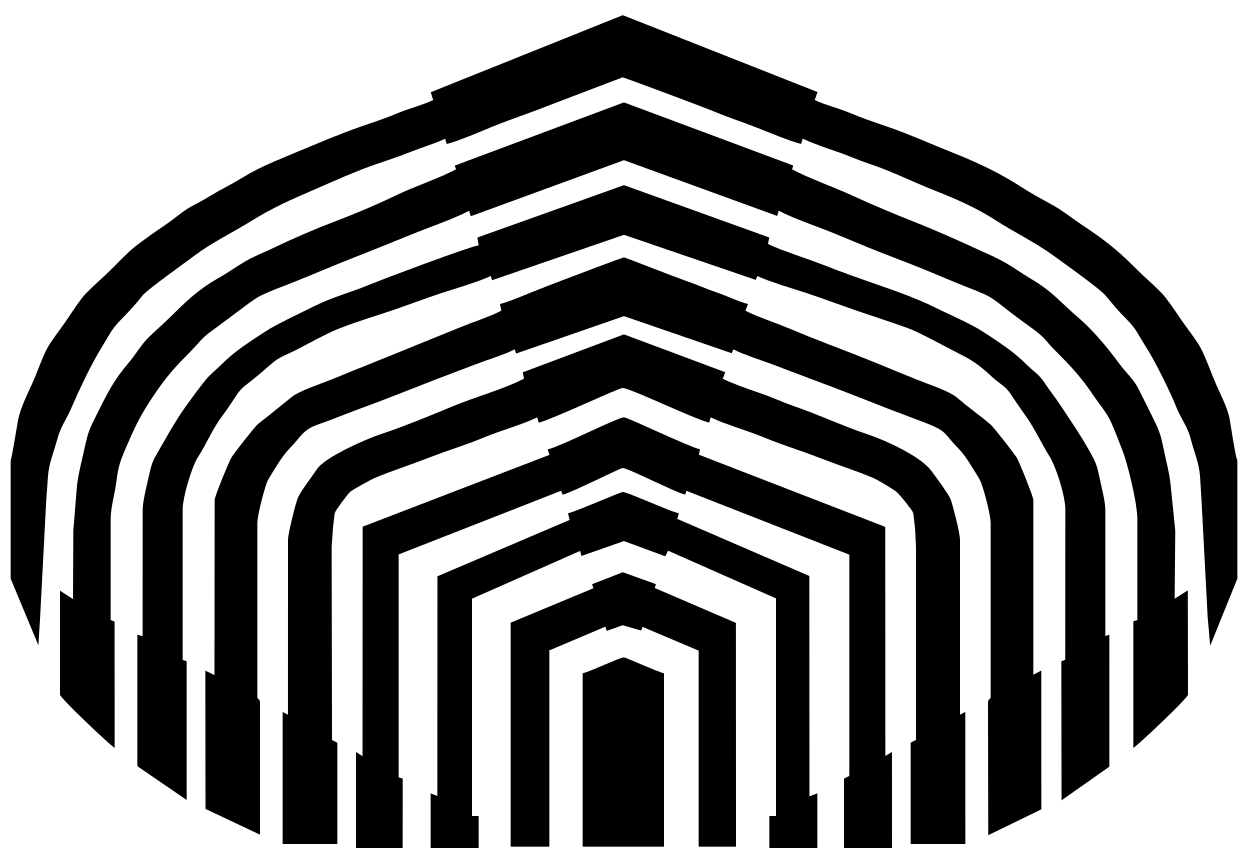
\includegraphics
			[width=.35\marginparwidth]
			{/home/jhonny/git/LaTeX-University/usb-logo.png}\\
		Universidad Simón Bolívar\\
		Caracas, Venezuela\\
		\end{center}
		\end{minipage}
		}
	{
	\Large\headfont
		\MyTitle
	\par
	}
	\smallskip
	\Asignatura\par
	\smallskip
	\@author,\ \today.
	\end{flushleft}
	\vskip 1.5\baselineskip
	}
\makeatother

\usepackage[final]{listings} 
\lstset
{
numbers=left, numberstyle=\tiny\ttfamily, stepnumber=2, numbersep=5pt, 
basicstyle=\ttfamily, 
stringstyle=\ttfamily,
commentstyle=\itshape,
breaklines=true,
postbreak=\mbox{$\hookrightarrow$\enspace},
columns=flexible
}

\usepackage{caption} 
\captionsetup
{
font={rm},
justification=raggedright,
singlelinecheck=false,
skip=3pt
}

\usepackage[explicit]{titlesec}

\titleformat{\section}[hang]
	{\flushleft\headfont}
	{\addfontfeatures{Numbers=Lining}\thesection}
	{1em}
	{\addfontfeatures{LetterSpace=5}\MakeUppercase{#1}}
	[]
\titlespacing*{\section}
	{0em}
	{1.5\baselineskip}
	{.5\baselineskip}
\titleformat{\subsection}
	{\flushleft\sffamily}
	{\addfontfeatures{Numbers=Lining}\thesubsection}
	{.5em}
	{#1}
	[]
\titlespacing*{\subsection}
	{0em}
	{1\baselineskip}
	{1\baselineskip}
\titleformat{\paragraph}[runin]
	{\scshape}
	{}
	{0em}
	{\MakeLowercase{#1}}
	[.]
\titlespacing*{\paragraph}
	{0em}
	{1\baselineskip}
	{5pt}

\let\oldtoc\tableofcontents
\renewcommand
{\tableofcontents}
{\marginpar{\bigskip\oldtoc}}
\usepackage{titletoc}

\titlecontents{section}
	[0em]
	{\vspace{0pt}}
	{\contentsmargin{0pt}}
	{\contentsmargin{0pt}}
	{\contentspage}
	[\vspace{.3em}]
\titlecontents{subsection}
	[1.5em]                              
	{\vspace{0pt}}
	{\contentsmargin{0pt}\small}
	{\contentsmargin{0pt}\small}        
	{\small\contentspage}                 
	[\vspace{.3em}]

\usepackage{fancyhdr}

\renewcommand{\headrulewidth}{0pt}
\setlength{\headheight}{14pt}

\pagestyle{fancy}
\fancyhf{}
\fancyhead
	[L]
	{
	\ifodd\value{page}\MyTitle\else\Asignatura\fi
	}
\fancyhead[R]{\thepage}
\fancypagestyle
	{plain}
	{
	\fancyhead[R]{}
	\fancyhead[L]{}
	\fancyfoot[R]{}%
	\fancyfoot[L]{}
	\fancyfoot[C]{}
	}

\usepackage[thmmarks]{ntheorem}
  % \usepackage[thmmarks]{ntheorem}
  % 	\theoremstyle{plain}
  % 	\theoremindent0cm
  % 	\theorempreskip{0cm}
  % 	\theorempostskip{0cm}
  % 	\theoremheaderfont{\hspace*{\parindent}\upshape}
  % 	\theorembodyfont{\itshape}
  % 	\theoremseparator{.}
  % 	\newtheorem{teo}{Teorema}[section]
  % 	\newtheorem{cor}{Corolario}[teo]
  % 	\newtheorem{prop}{Proposición}[section]
  % 	\newtheorem{lem}{Lema}[section]
  % 	\theoremstyle{nonumberplain}
  % 	\theoremheaderfont{\normalfont}
  % 	\theorembodyfont{\upshape}
  % 	\newtheorem{proof}{Demostración}
  % 	\theoremstyle{plain}
  % 	\theorempreskip{1em}
  % 	\theorempostskip{1em}
  % 	\theoremheaderfont{\upshape}
  % 	\theorempostwork{\noindent}
  % 	\newtheorem{definition}{Definición}[section]

\theoremstyle{plain}
\theorempreskip{\medskipamount}
\theorempostskip{\medskipamount}
\theorembodyfont{\upshape}
\theoremseparator{.}
{
\theoremheaderfont{\itshape}
\newtheorem{definition}{Definición}
}
{
\theoremheaderfont{\scshape}
\newtheorem{theorem}{Teorema}
}


\title{Tercer Parcial: Límites y Derivadas}
\author{Jhonny Lanzuisi,\\ 1510759}
\asignatura{Introducción a la teoría de anillos}

\begin{document}

\maketitle
\tableofcontents

% \tikzset{every picture/.style={line width=0.75pt}} %set default line width to 0.75pt        
\noindent
Los ejercicios se encuentran hola la misma numeración que el parcial originaa
por lo que se omiten los enunciados.\footnote{Los enunciados se pueden consultar en} 
\section{Primer ejercicio}
Queremos ver que el $ \lim_{x\to a} g(x)=L$. Dado $\epsilon =0$ sabemos \textit{a}$a$ que existen números reales
$\delta_1,\delta_2$ correspondientes a $f,h$ (respectivamente) tales que, si $x\in B(a,\delta_1)$ entonces
\[
	-\epsilon<f(x)-L<\epsilon
\]
y si $x\in B(a,\delta_2)$ entonces
\[
	-\epsilon<h(x)-L<\epsilon.
\]
Tomemos ahora $\delta=\min\{\delta_1,\delta_2,M\}$. Entonces la bola $B(a,\delta)$ esta contenida 
en las tres bolas de mismo centro pero de radios $\delta_1,\delta_2,M$ (ver la figura 1).%
%
%\marginnote{\centering Figura 1\\
	%\begin{tikzpicture}[x=0.75pt,y=0.75pt,yscale=-1,xscale=1,scale=.9]
	 %\path (0,300); %set diagram left start at 0, and has height of 300

%%Shape: Axis 2D [id:dp5087658793445884] 
%\draw  (55.5,241.5) -- (241,241.5)(71,91) -- (71,258.5) (234,236.5) -- (241,241.5) -- (234,246.5) (66,98) -- (71,91) -- (76,98)  ;
%%Straight Lines [id:da44085950811799] 
%\draw    (140.67,235.33) -- (140.67,248) ;
%%Straight Lines [id:da6831458041731795] 
%\draw    (170.44,237) -- (170.33,246.33) ;
%%Straight Lines [id:da882572117477251] 
%\draw    (190.44,237) -- (190.33,246.33) ;
%%Straight Lines [id:da24792462205657406] 
%\draw    (220.44,237) -- (220.33,246.33) ;
%%Straight Lines [id:da5487334614763701] 
%\draw    (110.44,236.67) -- (110.33,246) ;
%%Curve Lines [id:da7229552911253749] 
%\draw [color={rgb, 255:red, 208; green, 2; blue, 27 }  ,draw opacity=1 ]   (15.56,202.17) .. controls (46.33,228.67) and (222.84,133.17) .. (258.57,169.33) ;
%%Curve Lines [id:da7345588134660965] 
%\draw [color={rgb, 255:red, 245; green, 166; blue, 35 }  ,draw opacity=1 ]   (19.09,192.83) .. controls (66.14,162) and (166.6,270) .. (262.1,214) ;
%%Curve Lines [id:da5640137069572859] 
%\draw    (11.67,178.67) .. controls (59.77,232.67) and (231.68,150) .. (277.67,202.67) ;
%%Shape: Boxed Line [id:dp8072285224398166] 
%\draw    (75.72,230.94) -- (66.39,231.06) ;
%%Shape: Boxed Line [id:dp5891617412768961] 
%\draw    (75.72,158.28) -- (66.39,158.39) ;
%
%% Text Node
%\draw (141.67,258.67) node  [font=\small]  {$a$};
%% Text Node
%\draw (192.33,228.67) node  [font=\footnotesize]  {$M$};
%% Text Node
%\draw (170,258.33) node  [font=\footnotesize]  {$\delta _{1}$};
%% Text Node
%\draw (220.33,259) node  [font=\footnotesize]  {$\delta _{2}$};
%% Text Node
%\draw (181.43,260.91) node [anchor=north west][inner sep=0.75pt]  [font=\footnotesize,rotate=-33.22,xslant=-0.06] [align=left] {=};
%% Text Node
%\draw (195.67,272.33) node  [font=\footnotesize]  {$\delta $};
%% Text Node
%\draw (262.67,152.57) node [anchor=north west][inner sep=0.75pt]  [font=\small,color={rgb, 255:red, 208; green, 2; blue, 27 }  ,opacity=1 ]  {$h( x)$};
%% Text Node
%\draw (265,217.4) node [anchor=north west][inner sep=0.75pt]  [font=\small,color={rgb, 255:red, 245; green, 166; blue, 35 }  ,opacity=1 ]  {$f( x)$};
%% Text Node
%\draw (281,187.4) node [anchor=north west][inner sep=0.75pt]  [font=\small,color={rgb, 255:red, 0; green, 0; blue, 0 }  ,opacity=1 ]  {$g( x)$};
%% Text Node
%\draw (110,255) node  [font=\footnotesize]  {$-\delta $};
%% Text Node
%\draw (33.33,152.9) node [anchor=north west][inner sep=0.75pt]  [font=\footnotesize]  {$\epsilon -L$};
%% Text Node
%\draw (27.67,224.23) node [anchor=north west][inner sep=0.75pt]  [font=\footnotesize]  {$-\epsilon -L$};
%\end{tikzpicture}	
%}[3em]

Si $x\in B(a,\delta)$ se tiene que, por un lado
\begin{align}\label{eq:1}
	f(x)\leq g(x)\leq h(x)
\end{align}
y, por otro lado,
\begin{align}\label{eq:2}
	\left\lvert f(x)-L \right\rvert <\epsilon,\quad \left\lvert h(x)-L \right\rvert<\epsilon.
\end{align}

Juntando~(\ref{eq:1}) y~(\ref{eq:2}) se obtiene
\[
	-\epsilon<f(x)-L<g(x)-L<h(x)-L<\epsilon,
\]
de donde se sigue
\[
	-\epsilon<g(x)-L<\epsilon.
\]
Y se tiene entonces que $ \lim_{x\to a}g(x)=L $.

\section{Segundo Ejercicio}%


Tomemos un $a\in\mathbb{R}$. Por la negación del corolario~\ref{cor:contseq}, basta con conseguir
alguna sucesión real $\{ x_n \}$ convergente a $a$ para la cual se tenga que
\begin{align}\label{eq:3}
	f(a)\neq \lim_{n \to \infty}  f(x_n).
\end{align}
Dividiremos la demostración en dos casos:
\begin{description}
	\item[Si $a$ es racional.]
		En este caso tomemos un número $\alpha$ irracional. Entonces la sucesión
		$\{ x_n \}$ dada por
		\[
			\sum x_n= \int \frac{\alpha}{n} + a
		\]
		es tal que $x_n\to a$ cuando $n\to\infty$. 
		Pero como $\alpha$ es irracional se sigue que $\alpha/n $ también lo es
		de donde $\alpha/n + a$ es también irracional 
		(pues la suma de un número racional y uno irracional siempre es irracional).

		Se tiene entonces que, como todos los $x_n$ son irracionales,
		\[
			f(x_n)=0\quad\text{para todo $n\in\mathbb{N}$},
		\]
		pero $f(a)=1$.
		
	\item[Si $a$ es irracional.] En este caso, consideremos el conjunto $A$ de todos
%\marginnote{Sucesión $x_n$ convergente a $a$.\\
	%\begin{tikzpicture}[x=0.75pt,y=0.75pt,yscale=-1,xscale=1]
%%uncomment if require: \path (0,300); %set diagram left start at 0, and has height of 300
%
%%Straight Lines [id:da33306306965494015] 
%\draw    (100,122) -- (267.67,122) ;
%%Straight Lines [id:da32365339533662774] 
%\draw    (259.67,112.67) -- (259.67,131.33) ;
%%Straight Lines [id:da38315840975758275] 
%\draw    (109.67,112) -- (109.67,130.67) ;
%%Straight Lines [id:da22227714468718218] 
%\draw    (247.11,117.33) -- (247,126.67) ;
%%Straight Lines [id:da2882754094691373] 
%\draw    (150.78,117) -- (150.67,126.33) ;
%%Straight Lines [id:da8739024195762054] 
%\draw    (198.44,117) -- (198.33,126.33) ;
%%Straight Lines [id:da3419128535313456] 
%\draw    (128.78,117.33) -- (128.67,126.67) ;
%
%% Text Node
%\draw (274.67,136.67) node  [font=\small]  {$a+1$};
%% Text Node
%\draw (110,136.67) node  [font=\small]  {$a$};
%% Text Node
%\draw (247.67,132) node  [font=\scriptsize]  {$x_{1}$};
%% Text Node
%\draw (151.67,132) node  [font=\scriptsize]  {$x_{3}$};
%% Text Node
%\draw (199.67,133.33) node  [font=\scriptsize]  {$x_{2}$};
%% Text Node
%\draw (129.67,132.33) node  [font=\scriptsize]  {$x_{4}$};
	%\end{tikzpicture}
%}
		los racionales pertenecientes al intervalo $(a,a+1)$. Este conjunto $A$
		es númerable, por lo que podemos ordenarlo de manera descendente. Se obtiene
		así una sucesión $\{ x_n \}$ de números racionales, cada vez mas pequeños, que
		convergen a $a$ (si este no fuese el caso, entraríamos en contradicción con el hecho
		de que los racionales son densos en cualquier intervalo de $\mathbb{R}$).

		Como todos los $ x_n $ son racionales, se sigue que
		\[
			f(x_n) = 1\quad\text{para todo $n\in\mathbb{N}$}
		\]
		pero $f(a)=0$.
\end{description}

Entonces, sin importar cual sea el punto $a$ siempre se puede encontrar una
sucesión para la cual ocurre~(\ref{eq:3}) y se sigue que $f$ no es continua en \emph{ningun} $a$.

% \begin{marginfigure}
% 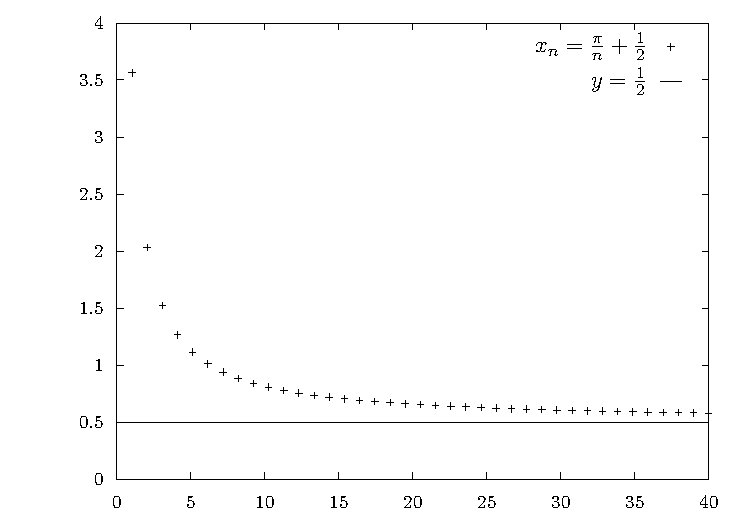
\includegraphics[width=\linewidth]{pics/out}
% \caption{Ejemplo con $\alpha=\pi$ y $a=1/2$. La sucesión $x_n$ (morada) converge a
% $1/2$ (línea verde).}
% \end{marginfigure}

\section{Tercer Ejercicio}%
%\marginnote{\centering Figura 3\\
%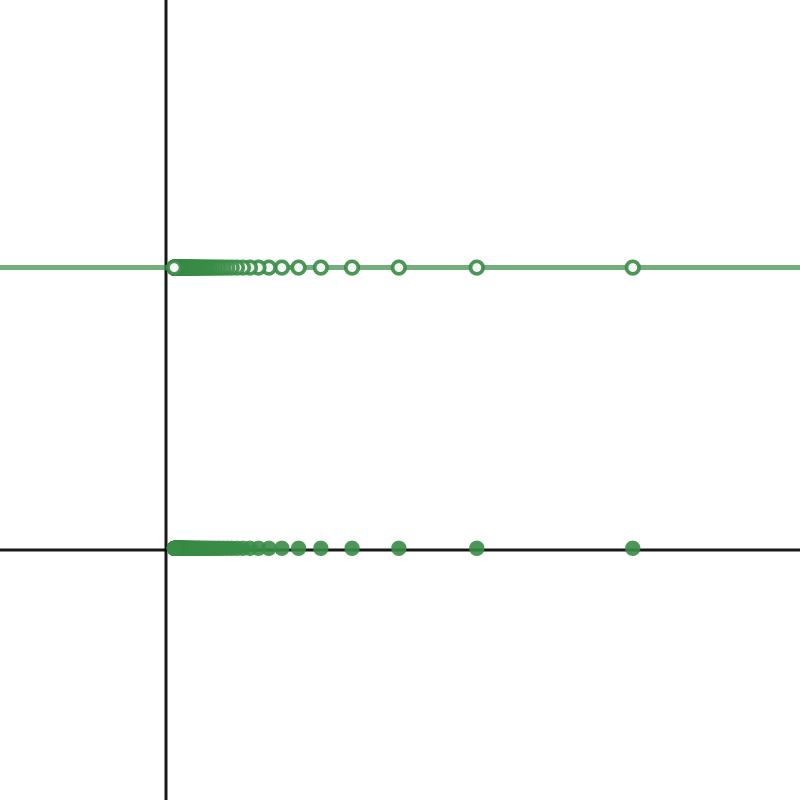
\includegraphics[scale=.2]{pics/g3.png}\\
%Gráfico de la función $g$, los puntos `vacios'
%representan los saltos de $g$ en los números
%de la forma $1/n$.
%}
Sea $\mathcal{A}=\left\{ \{0\}\cup \left\{ 1/n \right\} \right\}(n\in\mathbb{N})$. Consideremos la función $g$ dada por 
\[
	g(x)=\begin{cases}
		1 &\text{si $x\notin \mathcal{A}$},\\
		0 &\text{si $x\in\mathcal{A}$}.
	\end{cases}\qquad\text{(figura 3)}
\]
Esta función es discontinua en los puntos de $\mathcal{A}$ dado que tiene \emph{saltos} en
esos puntos.%

 Por otro lado, si $x\notin\mathcal{A}$ entonces $g(x)$ es continua puesto que 
siempre se puede encontrar un entorno del punto $x$ que no contiene ningún
número de la forma $1/n$: si $x>1$ entonces esto es evidente, si $x<1$ entonces existe un entero $m$ tal que
\[
	x\in\left(\frac 1m, \frac{1}{m+1} \right).
\]
Es claro que en este intervalo no hay ningún número de la forma $1/n$, por lo tanto en este
intervalo la función $g$ es constantemente igual a $1$, y se sigue que $g$ es continua en $x$.

\section{Cuarto Ejercicio}%
Para ver que $f$ es continua en $a$, queremos ver que
\[
	\lim_{x\to a} f(x)=f(a).
\]
Esto en efecto es así. Primero notemos que
\[
	f(0)=f(0+0)=f(0)+f(0)-o
\]
implica $f(0)=0$. Como $f$ es continua en $0$ esto nos dice que
$ \lim_{x\to0} f(x)$ es igual a $0$.

Ahora,
\allowdisplaybreaks
\begin{align*}
	\lim_{x\to a} f(x) &= \lim_{h\to 0} f(a+h)&\quad\text{(por el teorema~\ref{teo:limcambvar})}\\
			   &= \lim_{h\to 0} \bigl(f(a)+f(h)\bigr)&\quad\text{(por la definición de $f$)}\\
			   &=f(a)+0&\\
			   &=f(a).&
\end{align*}
	
\section{Quinto Ejercicio}%
Como todas las funciones constantes son tales que su derivada en cualquier punto es cero,
basta con demostrar que $f'(a)=0$ para todo $a$ y tendremos que $f$ es constante.

Sea $a\in\mathbb{R}$. Entonces
\begin{align}\label{eq:4}
	f'(a)= \lim_{h\to 0} \frac{f(a+h)-f(h)}{h} 
\end{align}
es la derivada de $f$ en $a$. Pero notemos que
\[
	-a^2<f(a+h)-f(h)<a^2
\]
por nuestra hipótesis acerca de $f$. De la ecuación anterior se sigue que
\[
	-\frac{a^2}{h}< \frac{f(a+h)-f(h)}{h}< \frac{a^2}{h},
\]
y el primer ejercicio asegura que el límite en~(\ref{eq:4}) es igual al límite de
\[
	\frac{a^2}{h} 
\]
que es claramente cero.

Entonces $f'(a)=0$ para todo $a$ y $f$ es una función constante.

\section{Sexto Ejercicio}%
Construiremos una $f$ que cumple con la condición pedida concatenando
semicircunferencias de la forma
\[
	y=\sqrt{r^2-(x-c)^2},
\] 
donde $r$ es el radio y $c$ el centro.

Las semicircunferencias son funciones continuas 
en todos sus puntos y derivables en todos menos\nota{Otra prueba pa ve que tal} los extremos. Por lo tanto,
si colocamos los extremos de las semicircunferencias de tal forma
que coincidan con los puntos de la forma $1/n$ obtendremos
una función con la condición pedida.
%
%\marginnote{\centering Figura 4\\
%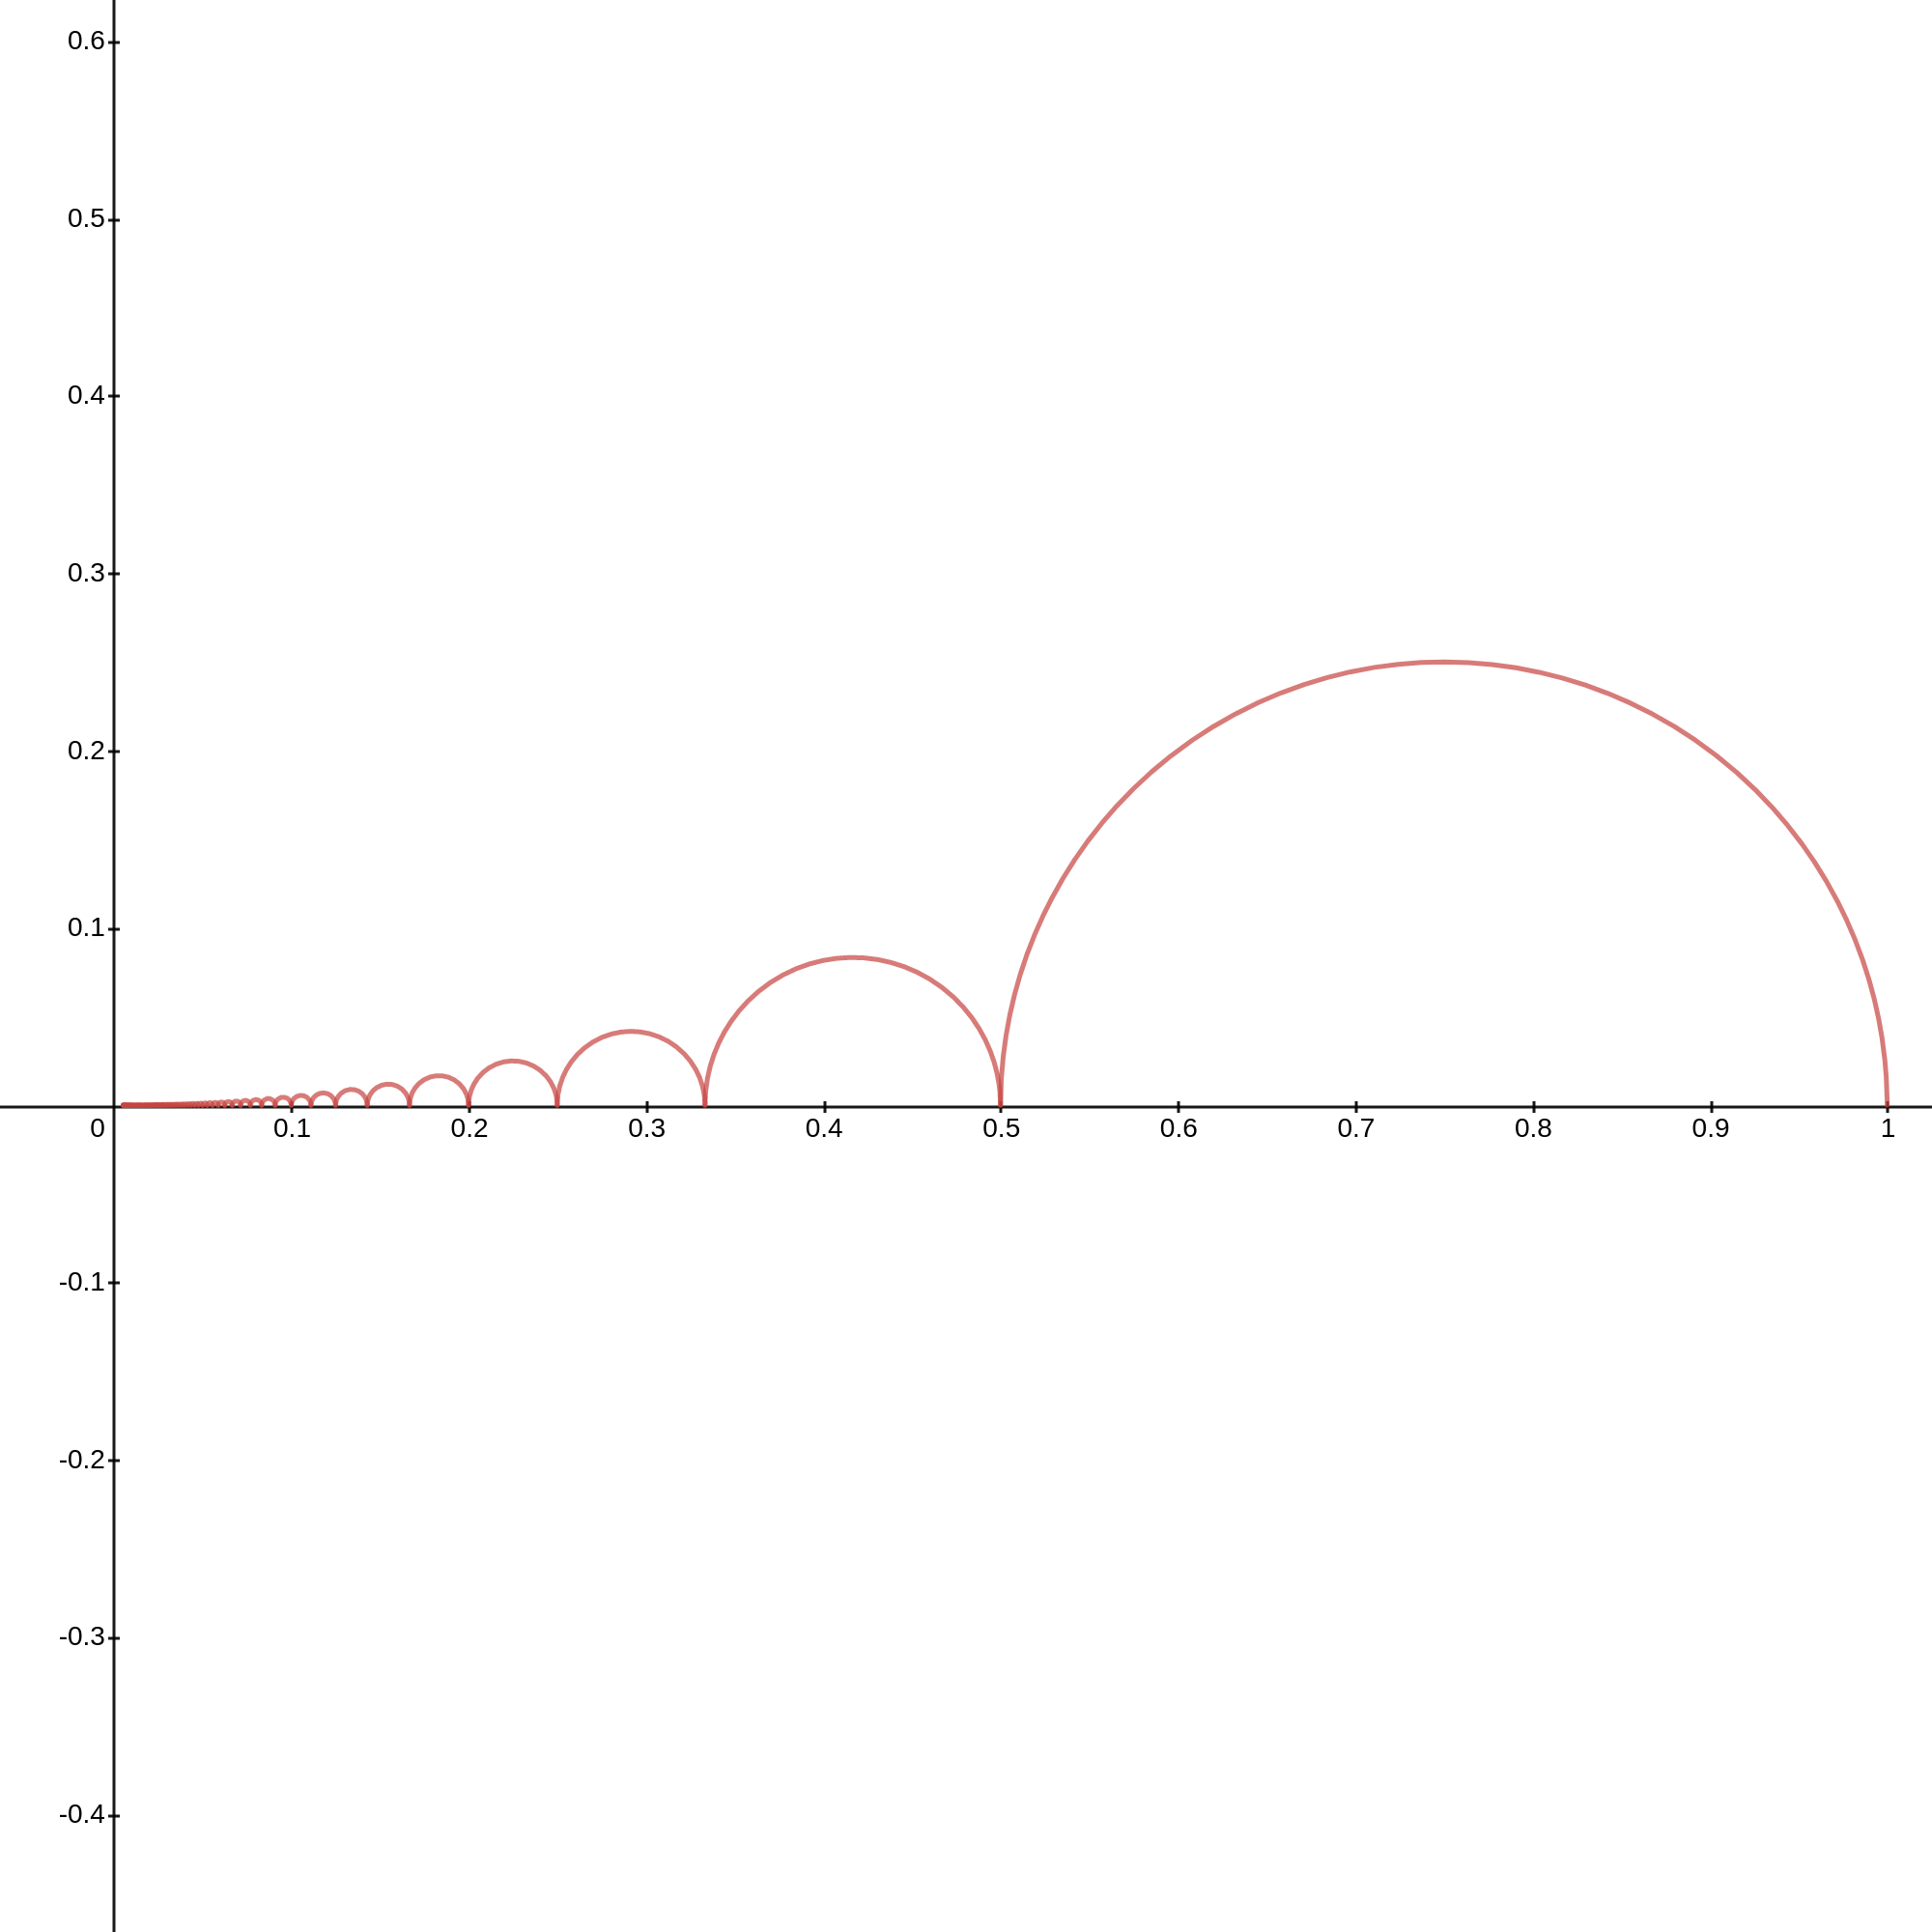
\includegraphics[scale=.1]{pics/g4.png}\\
%Una función $f$ que es continua y diferenciable en todos
%los puntos excepto los de la forma $1/n$.

Para que los extremos queden en el lugar correcto debemos
colocar los centros en el punto medio entre $1/n$ y $1/(n+1)$,
esto es,
\[
	c= \frac{1}{2} \left( \frac{1}{n} + \frac{1}{n+1} \right) (n=1,2,\dots).
\]
Además, los radios deben ser del tamaño correcto:
\[
	r=n-c.
\]
Con la información que tenemos podemos construir la función
$f$ a trozos (figura 4):
\[
	f(x)= \begin{cases}
		\sqrt{r^2-(x-c)^2} &\text{si $\dfrac{1}{n+1}\leq x< \dfrac 1n $}\quad (n=1,2,\dots).
	\end{cases}
\]
Es decir, el primer trozo de $f$ (para el intervalo $1/2\leq x<1$) viene dado por
\[
	f(x)=\sqrt{\biggl(1- \frac{1}{2}\bigl(1+ \frac{1}{2}\bigr)\biggr)^2 - 	\biggl(x-\frac{1}{2}\bigl(1+ \frac{1}{2}\bigr)\biggr)^2}
\]
o, que es lo mismo, por
\[
	f(x)=\sqrt{(1-3/4)^2-(x-3/4)^2};
\]
y así sucesivamente para $n=2,3,\dots$.%

Nuestra función $f$ así definida cumple con el razonamiento dado
en el segundo párrafo. El gráfico ayuda aún más a convencerse de este hecho.

\section{Séptimo Ejercicio}%
Hagamos
\[
	g(x)= \frac{f(x)-f(a)}{x-a} .
\]
Entonces queremos ver que $g'(x)$ es positiva, pues eso nos dará que
el cociente es creciente.

Podemos usar el criterio del cociente para hallar la derivada de $g$:
\[
	g'(x)= \frac{(x-a)(f'(x)-f'(a))-(f(x)-f(a))}{(x-a)^2} .
\]
Primero que todo, es claro que $(x-a)^2>0$. Ahora como $a$ es el extremo izquierdo del intervalo se tiene
que para todo $x\in(a,b)$ se cumple $x>a$ y $x-a>0$. Como $f''>0$ se sigue que $f'$ es creciente y entonces
$f'(x)-f'(a)>0$ y el producto $(x-a)(f'(x)-f'(a))$ es positivo. Y como $f(x)-f(a)<0$ se sigue que $g'(x)>0$\nota{esto es lo único que se me ocurrió para este ejercicio. Estoy casi seguro que no es la resolución correcta}
.

\section{Resultados Utilizados}

\begin{cor}\label{cor:contseq}
	Sea $f\colon A\subset\mathbb{R}\to\mathbb{R}$. Entonces $f$ es continua en un punto $a$ si, y solo si,
	para toda sucesión $\{ x_n \}$ de puntos en $A$ tal que  
	$ \lim_{n \to \infty}x_n=a, $
	se tiene que $ \lim_{n \to \infty} f(x_n)=f(a)$.\nota{El corolario fue tomado de la guia de la profesora Marcantognini pag. 108}
\end{cor}
\begin{teo}\label{teo:limcambvar}
	Sea $f\colon A\subset\mathbb{R}\to\mathbb{R}$. Entonces
	\[
		\lim_{x\to v} f(x)= \lim_{h\to 0} f(v+h)
	\]
	siempre que el límite de la izquierda exista.
\end{teo}
\begin{proof}
	Sea $ \lim_{x\to v} f(x)=L$, entonces dado $\epsilon>0$ existe un $\delta$ tal que si
	\[
		\left\lvert x-v \right\rvert<\delta\quad\text{entonces}\quad
		\left\lvert f(x)-L \right\rvert<\epsilon.
	\]
	Si hacemos $h=x-v$, entonces lo anterior se convierte en
	\[
		\left\lvert h \right\rvert<\delta\quad\text{entonces}\quad
		\left\lvert f(h+v)-L \right\rvert<\epsilon,
	\]
	que significaa
	\[
	\lim_{h\to 0} f(v+h)=L.
	\]
\end{proof}
% \printbibliography[
% heading=bibintoc,
% title={Referencias}
% ]
\end{document}
